\documentclass[letterpaper,12pt]{article}
\usepackage[utf8]{inputenc}
\usepackage[bottom]{footmisc}
\usepackage{graphicx}
\usepackage{amsmath}
\usepackage{amsthm}
\usepackage{amscd}
\usepackage{amssymb}
\usepackage{latexsym}
\usepackage{upref}
\usepackage[hidelinks]{hyperref}
\usepackage{cite}

\setlength{\textwidth}{6.4in}
\setlength{\textheight}{9.5in}
\setlength{\topmargin}{-1in}
\addtolength{\headheight}{0.0675in}
\setlength{\oddsidemargin}{0.2in}
\setlength{\evensidemargin}{0.2in}

\begin{document}

    \title{
        A Deep Learning Approach to Solving Hyperbolic PDEs\\
    }
    \author{%
        Thompson, J.
    }
    \date{\today}
    \maketitle

    \begin{abstract}
        In this project, we examine a deep learning approach to solving various hyperbolic equations, including 
        (but not limited to) a basic advection equation and the one-dimensional inviscid Burgers equation.
        Such equations arise naturally in the study of fluid and traffic flows and are solvable via traditional 
        finite difference approaches. Numerical solutions are therefore readily available (or may be easily generated),
        and so the problem of data collection for deep learning is well-mitigated.
    \end{abstract}


    \section{Background}\label{sec:background}
    Recent advancements in the field of machine learning have led to the development of Physics-Informed Neural 
    Networks (PINNs), wherein a neural network is used as a solution surrogate to systems of partial differential 
    equations (PDEs). Such networks are typically trained from available sparse data; typically, the amount of data
    available to train a neural network is insufficient for a neural network to converge. However, by encoding the 
    governing PDE term into the network training process (either by including the PDE residual into network training as
    in a multi-objective approach or by some other scheme), recent empirical successes indicate that
    sparse data and/or specified boundary conditions provide sufficient convergence conditions for the neural network to
    successfully approximate the true PDE solution.\cite{raissi_physics-informed_2019} In fact, neural networks are 
    particularly well-suited to solve the inverse problem for PDEs - that is, to infer some unknown parameter of 
    function which is part of the original system of PDEs.\cite{lu_deepxde_2021} In this project, we propose to utilize
    PINNs to solve both the forward and inverse problem for two well-known hyperbolic PDEs. The first of these is a 
    standard advection equation, which is the simplest possible hyperbolic PDE:

    $$
    u_t + a u_x = 0
    $$

    \noindent for some constant $a$ and initial condition $u(x, 0) = u_0(x)$. The second equation we will examine is the
    inviscid Burgers' equation, which we obtain by letting $a = u$ from above:

    $$
    u_t + u u_x = 0
    $$

    \section{Proposed Methodology}\label{sec:proposed-methodology}

    In this project, we will utilize DeepXDE\footnote{
        Source code for this library may be found at
        \hyperlink{https://github.com/lululxvi/deepxde}{https://github.com/lululxvi/deepxde}
    }, a Python framework built on top of Tensorflow for scientific machine learning and physics-informed 
    learning.\cite{lu_deepxde_2021} DeepXDE solves PDEs by embedding the PDE residual term into the loss term of the
    neural network solution approximation. For the forward solution (i.e., with specified initial and boundary 
    conditions), the resulting neural network takes spatiotemporal data as input and outputs the predicted solution 
    value at each point. PINNs typically operate well with 1-3 hidden layers, though one aim of this project is to 
    determine which neural network architecture(s) lead to convergent system solutions. For the inverse problem, we will
    generate training data for both advection and inviscid Burgers' equations via known solutions for particular values
    of $a$ and initial condition $u_0(x)$ to determine these values only from sampled solution data.

    \begin{figure}[h]
        \centering
        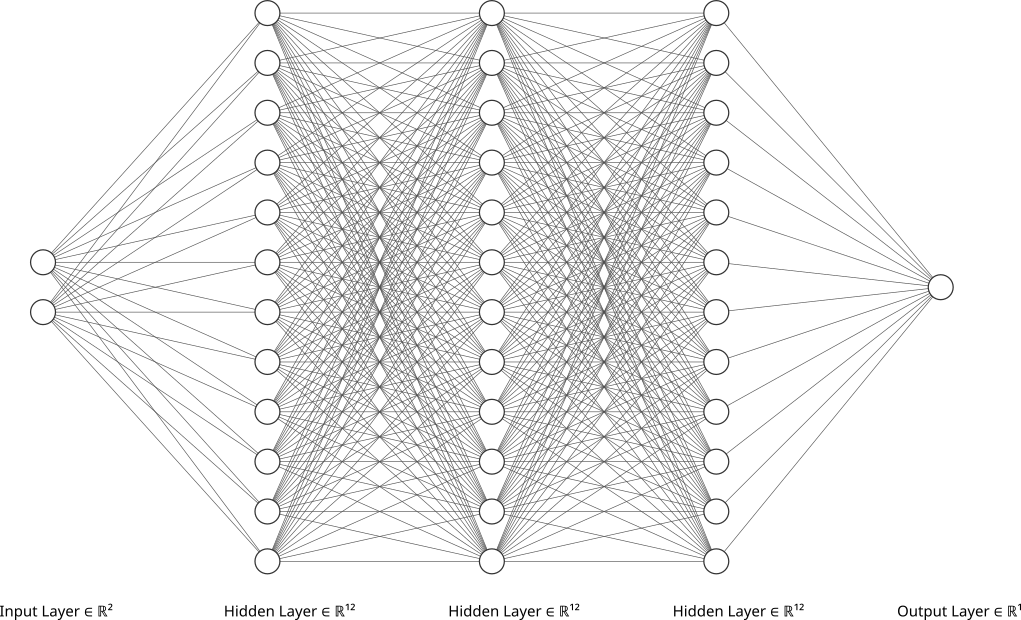
\includegraphics[width=0.75\textwidth]{nn.png}
        \caption{Proposed neural network architecture for hyperbolic PDE}
    \end{figure}

    \section{Goals and Objectives}\label{sec:goals}
    We hope to utilize neural networks to solve an advection and inviscid Burgers equation with a known reference 
    solution. Moreover, we hope to analyze the applicability of the learned equation to similar systems in order to 
    determine whether the trained neural network provides robustness and/or generalizability beyond that of the provided
    training data set. For the inverse problem in the advection equation, we will examine the trained network's ability 
    to predict values of $a$ from other initial conditions. Furthermore, if time allows, we will examine the utility
    of PINNs in solving the viscid Burgers' equation in both forward and inverse cases with residual-based
    adaptive refinement to account for the sharp front:

    $$
    u_t + u u_x = \nu u_{xx}
    $$

    \pagebreak
    \nocite{*}
    \bibliographystyle{plain}
    \bibliography{refs}


\end{document}
